\documentclass{article}

% if you need to pass options to natbib, use, e.g.:
% \PassOptionsToPackage{numbers, compress}{natbib}
% before loading nips_2016
%
% to avoid loading the natbib package, add option nonatbib:
% \usepackage[nonatbib]{nips_2016}

% \usepackage{nips_2017}

% to compile a camera-ready version, add the [final] option, e.g.:
\usepackage[final]{nips_2017}

\usepackage[utf8]{inputenc} % allow utf-8 input
\usepackage[T1]{fontenc}    % use 8-bit T1 fonts
\usepackage{hyperref}       % hyperlinks
\usepackage{url}            % simple URL typesetting
\usepackage{booktabs}       % professional-quality tables
\usepackage{amsfonts}       % blackboard math symbols
\usepackage{nicefrac}       % compact symbols for 1/2, etc.
\usepackage{microtype}      % microtypography

\usepackage{amsmath}	% for \begin{align}
\usepackage{graphicx}	% for \includegraphics{filename}
\usepackage{subcaption}	% for \begin{subfigure}[t]{0.5\textwidth}

\newcommand{\bb}[1]{\boldsymbol{#1}}

\title{Adversarial Zero-Shot Learning}

% The \author macro works with any number of authors. There are two
% commands used to separate the names and addresses of multiple
% authors: \And and \AND.
%
% Using \And between authors leaves it to LaTeX to determine where to
% break the lines. Using \AND forces a line break at that point. So,
% if LaTeX puts 3 of 4 authors names on the first line, and the last
% on the second line, try using \AND instead of \And before the third
% author name.

\author{
	Shihui Li, Yu-Hsiang Lin, Kangyan Zhou
		%\thanks{Use footnote for providing further information about author (webpage, alternative address)---\emph{not} for acknowledging funding agencies.}
		\\
	Language Technologies Institute\\
	Carnegie Mellon University\\
	Pittsburgh, PA 15213 \\
	\texttt{\{shihuil,yuhsianl,kangyanz\}@andrew.cmu.edu} \\
	%% examples of more authors
	%% \And
	%% Coauthor \\
	%% Affiliation \\
	%% Address \\
	%% \texttt{email} \\
	%% \And
	%% Coauthor \\
	%% Affiliation \\
	%% Address \\
	%% \texttt{email} \\
}

\begin{document}

\maketitle

\begin{abstract}
In Zero-shot learning(ZSL), how to learn discriminative features for fine-grained classes is a main challenge. In this paper, we propose a novel model: semantic adversarial autoencoder(SAAE) to solve ZSL problem. This approach is based on a semantic autoencoder(SAE), which projects image representation onto the space of semantic features. We incorporate a discriminator for semantic representations to  strengthen the discriminative power of the model. The result of experiments on two standard datasets shows that our model is able to outperform other baseline models, especially in generalized ZSL scenario. 
\end{abstract}

% ----------------------------------------------------
% ----------------------------------------------------

\section{Introduction}

Zero-shot learning has been an active research topic in the field of image classification. It simulates how people learn things: when people see an unfamiliar object, they use existing knowledge and try to evaluate the new object. Ideally, a large-scale image classification system should be able to recognize novel categories based on its previous training experience. One of the main challenges for object recognition is the lack of sufficient annotations for all possible concepts. This problem becomes even more severe when we target at the task of fine-grained classification because the annotation is more expensive and the number of fine-grained classes is huge. Realizing this limitation, researchers resort to additional information, for example, textual description, to solve this problem.  

On the other hand, autoencoder has shown its great express power to present complicate distributions such human faces, natural sceneries and natural language. It is able to convert complicated real world data distributions, e.g. text features, to very well-formed low dimension. Many studies have shown that after applying autoencoder techniques, the learned latent feature space often has clear semantic meanings. For example, in \cite{makhzani2015adversarial}, all the digits can be well embedded into a low-dimensional manifold such that similar digits will have smaller distance within that manifold.

 \par 

The fundamental problem of ZSL is to extract semantically meaningful feature embeddings that could bridge the gap between similar image/text features and fine-grained classes. Autoencoder becomes an ideal option for this task because it can automatically learn important features. In \cite{kodirov2017semantic}, they present a novel solution to zero-shot learning--Semantic AutoEncoder(SAE). Taking the encoder-decoder paradigm, an encoder aims to project a visual feature vector into the semantic space as in the existing zero-learning shot models and the decoder should be able to reconstruct the original visual feature. Their results show that under this framework, the learned projection function from the seen classes is able to generalize better to the new unseen classes. One shortcoming of this model is that the encoder tends to learn similar features across multiple classes, which is disappointing for the task of fine-grained classification. 

Inspired by these models, we propose an Semantic Adversarial AutoEncoder(SAAE). In our model, we have an encoder that projects a visual feature vector into the semantic space and a decoder that decodes and reconstructs the original visual features. Besides, we incorporates a discriminator as in \cite{makhzani2015adversarial} to ensure that generating from any part of prior space results in meaningful samples.

Two types of discriminators will be discussed in this project, one is independent from semantic space and the other is dependent from semantic space. 

% In this project we plan to explore how to develop an effective transfer learning algorithm, with focus on zero-shot learning and its combination with several popular deep learning methods, such as convolutional neural network, attention models, and Adversarial training, to detect unseen objects only with text description. \\
% Zero-shot learning consists in learning how to recognize new concepts by just having a description of them. State-of-the-art methods for zero-shot recognition formulate learning as a embedding problem of images and side information like text \cite{Elhoseiny2013}. We propose a model that can classify unseen categories from their textual description. Inspired by the fact that there is little supervision on text data, certain noise-cancelling techniques could be applied to improve the performance of our model.\\




% ----------------------------------------------------
% --------------------------------------------------


\section{Related Works}    
Considering that fine-grained categories might share some common knowledge, a common approach is to seek for an intermediate semantic representation that could connect seen and unseen classes. Human specified attributes are first explored to represent the discriminative properties shared among both seen and unseen categories in zero-shot learning\cite{torresani2010efficient, lampert2009learning}. One limitation of this method is that the creation of attributes still relies on human labors, making it difficult to scale up to meet large scale needs. \par 

%Other forms of semantic representations have been explored since then. \cite{torresani2010efficient} employs the idea of using object detectors as the basic representations of images and the semantic concept is trained by using the entire image. \cite{mensink2014costa} attempts to capture the semantic relevance of two concepts by the co-occurrence of words.  In \cite{mensink2014costa, romera2015embarrassingly}, the authors assume that the classifier for an unseen class can be presented as a linear combination of seen class classifiers.

Apart from handcrafting attributes, another scheme is to directly use the online textual document as the additional information source. \cite{Elhoseiny2013} is one of the first works to use Wiki documents as text attributes. \cite{Ba_2015_ICCV} proposed a model that changes both the ways of extracting features from images and text domains. More specifically, the image features are extracted from the activation layer of a convolutional neural network(CNN), and then go through a linear projection layer to reduce dimensions. The input text, e.g. Wikipedia articles, is first converted to one-hot encodings of the words with their tf-idf scores, which can be viewed as attributes, and then fed into a multi-layer perceptron (MLP) to generate a deep representation, with the same dimension as the final image feature, and unique for each class. The final prediction is obtained by the dot product of the two generated features. Instead of learning an embedding space for each modalities, \cite{frome2013devise} learns joint image-word embeddings so as to embedding images and sentences into a common space.\\
	
	Another line of research is to improve the quality of the classification procedure. \cite{hariharan2012efficient} firstly proposed a SVM based classifier which takes the linear projection of both source and target domain data as the combined input. More recent works jointly project the class into an embedding space, and try to compute a compatability function $F(x, y)$ that tries to predict whether the image feature x is compatible with the embedded class feature y. Here each class is represented as a vector that contains the relevance scores of the class and a set of predefined attributes.  In \cite{akata2013label}, $F(x, y)$ takes a linear form as $F(x, y) = xWy$. \cite{xian2016latent} takes this idea one step further, where a set of $W_i$ is available for the the compatibility function $F(x, y)$, and the final prediction will choose the $W$ that can produce the highest score. This $W_i$ can be shared across different labels.  The method is called as latent embedding, since it learns a latent embedding space explicitly based on clustering. \cite{zhang2016zero} proposes a framework that generalizes deep learning embedding, label embedding, and latent embedding. \\ 
    
    Recently deep encoder-decoder has become popular for a variety of multi-modal problems. In \cite{kiros2014unifying}, they introduce an encoder-decoder pipeline that learns a multimodal joint embedding space with images and text and a novel language model for decoding distributed representations of the text semantic space. Their pipeline effectively unifies joint image-text embedding models with multimodal neural language models. \cite{kodirov2017semantic} takes a step further in multimodal model under the autoencoder paradigm. They proposed a novel zero-shot learning model based on a semantic autoencoder that uses a fast linear projection function and introduce an additional reconstruction objective function for learning a more generalisable projection function. \\ 


% 	In \cite{Elhoseiny2013}, during training, they learn the domain transfer function, $W$, from text domain to vision domain (in addition to feature extraction from text and image data). They use the approach from \cite{Kulis2011}. There is a measure of how much two feature vectors ($\bb{t}$ from text domain and $\bb{x}$ from vision domain) are similar to each other, based on $\bb{t}^{\top} W \bb{x}$. The training objective is basically that: (1) if $\bb{t}$ and $\bb{x}$ belong to the same class, their similarity should be more than a positive threshold (a margin), and (2) if $\bb{t}$ and $\bb{x}$ belong to the different classes, their similarity should be less than a negative threshold (a margin). It is trained with some regularization. (If the objective function is a direct/simple function of $\bb{t}^{\top} W \bb{x}$, it is non-convex for $\bb{t}$ and $\bb{x}$. That might be the reason that in \cite{Kulis2011} they use a more sophisticated formulation.)
	
% 	In fact, in \cite{Elhoseiny2013} during training they also need to learn the weight vectors $\bb{w}_i$, $i = 1, \dots, N_{sc}$ for ``seen classes'', but it seems that they do not describe how they learn these classifiers.
	
% 	They said that they ``learn'' the weight predictor (or the ``classifier regressor'') during training, but from their formulation it seems that as long as you have $\bb{w}_i$, then what the predictor does is that, given a new text vector $\bb{t}$, use $\bb{w}_i$ and Gaussian kernels (presumably with some fixed hyperparameters?) to compute (through an optimization problem) the predicted weight vector. So there doesn't seem to be any model parameters to learn here, but only works to do during inference time.
	
% 	During test time (inference), they give a clear constrained optimization problem to solve. What they try to optimize (in order to obtain the predicted weight vector $\bb{w}$ for an unseen-class text data $\bb{t}$) is basically:
% 		\begin{enumerate}
% 			\item Maximizing the similarity between $\bb{w}$ and $\bb{t}$ with respect to the domain transfer function $W$ (note that $W$ was trained using image feature $\bb{x}$ but here it is applied to weight vector $\bb{w}$ in image domain).
% 			\item Maximizing the log probability of having this $\bb{w}$ given $\bb{t}$ with respect to the weight predictor (and a given Gaussian prior).
% 			\item Minimizing the margin (well, it seems to be unbounded if you try to maximize the margin) of correctly labeling the seen classes all into negative side (they do not belong to the new class).
% 			\item Minimize the L2 regularizor.
% 		\end{enumerate}
% 		Their constraints are that all the seen images are classified as negative with some margin (done the slack variables, the margin, which are minimized).
	
	



% ----------------------------------------------------
% ----------------------------------------------------

% ----------------------------------------------------

% \subsection{Adversarial autoencoder}

% 	The adversarial autoencoder is a mixture of an autoencoder and a generative adversarial network. The input image $\bb{x}$ is encoded into $\bb{h}$ through encoder function $\bb{h} = f_{enc}(\bb{x})$. The reconstruction is performed by the conjugate decoder function $\tilde{\bb{x}} = f_{dec}(\bb{h})$. The autoencoder is trained to reconstruct the input image by minimizing the cross entropy loss,
% 		\begin{align}
% 			\textrm{loss} = -\bb{x}^{\top} \log \tilde{\bb{x}}.
% 		\end{align}
	
% 	The encoder also serves as the generator of the adversarial network, which generates negative samples with aggregated posterior distribution $q(\bb{h})$ that comes from the encoding distribution $q(\bb{h} | \bb{x})$ and the data distribution $p_d(\bb{x})$,
% 		\begin{align}
% 			q(\bb{h}) = \int q(\bb{h} | \bb{x}) p_d(\bb{x}) d \bb{x}.
% 		\end{align}
	
% 	A discriminator $D(\bb{z})$ gives the probability that $\bb{z}$ is a positive sample generated from a given and fixed prior distribution $r(\bb{z})$. The generator (the encoder) and discriminator are then jointly trained according to
% 		\begin{align}
% 			\min_{f_{enc}} \max_D \left\{ E_{\bb{z} \sim r(\bb{z})}[ \log D(\bb{z}) ] + E_{\bb{x} \sim p_d(\bb{x})}[ \log( 1 - D(f_{enc}(\bb{x})) ) ] \right\}.
% 		\end{align}
% 		That is, the generator (the encoder) is trained to generate samples mimicing the samples produced by the prior (such that the discriminator tends to classify it as positive samples from prior), and the discriminator is trained to classify the samples from prior as positive and those from generator as negative. The optimal solution is that the generator generates samples exactly according to the prior distribution (i.e.~$q(\bb{h}) \propto r(\bb{z})$), and the discriminator classifies samples from either the prior or the generator as positive samples with equal probabilities (e.g.~$D(\bb{z}) = D(f_{enc}(\bb{x})) = 1/2$).



% ----------------------------------------------------
% ----------------------------------------------------

\section{Semantic Adversarial Autoencoder}	
    
\subsection{Adversarial Autoencoder}
Adversarial autoencoder\cite{makhzani2015adversarial} is an antoencoder with a generator and a discriminator. In addition, a prior is chosen to regularize the hidden representation of the input data. During training time, the generator can generate positive samples given the prior, and the discriminator aims to discriminate the positive samples from the generator and the negative samples from the hidden layer of the autoencoder. This model structure often contributes to a clear boundary of the learned representations by simultaneously minimizing the reconstruction loss from a plain autoencoder, the loss of misclassifying negative samples from the discriminator, and the loss of failing to generate positive samples from the generator.

% ----------------------------------------------------
% ----------------------------------------------------

\subsection{Autoencoder models for ZSL}
Our SAAE model is an extension of semantic autoencoder(SAE)\cite{kodirov2017semantic}. In SAE, the inputs are the image features X and the attribute representations S of the corresponding class. The original optimization problem of the SAE is
    \begin{equation}
    \min_{W} || \bb{x} - W^{\top} W \bb{x} ||_2^2, \quad \text{s.t.} \;\; W \bb{x} = \bb{s},
    \end{equation}
   where W is the parameter in the autoencoder. This model enforces the hidden representation of images in the autoencoder to mimic the corresponding semantic representation. The loss is further relaxed to  
   \begin{equation}
   L_{\textrm{SAE}} = || \bb{x} - W^{\top} \bb{s}||_2^2 + \lambda || W \bb{x} - \bb{s} ||_2^2,
    \end{equation}
where a matching coefficient $\lambda$ is introduced here to control the importance of matching semantic space representation. (2) is a globally convex function, thus W can be solved via Bartels-Stewart algorithm\cite{lu1971solution}. 
    
    Based on SAE, We propose two architectures, explicit SAE and implicit SAE, which incorporate the idea of adversarial autoencoder. In one of them we draw positive samples from a Gaussian prior, and explicitly require the encoding $\bb{h}^c$ to approximate the semantic representation $ \bb{t}^c$. In this case, the prior serves as a regularizer, which is presented in Sec.~\ref{subsec:NoisePrior}. In the other, we directly use the text representation as positive samples drawn from some distribution that describes a class of data, and the code is trained by the adversarial net to match the text representation. In this case, the prior guides the generator (the encoder) to learn the code that is close to the semantic representation of text, which is presented in Sec.~\ref{subsec:TextPrior}.



% ----------------------------------------------------

\subsection{SAAE-exp}
\label{subsec:NoisePrior}
	
	The explicit SAAE\ref{fig:Architecturea} has an autoencoder that learns the encoding $\bb{h}^c$ of the input images $\bb{x}^c$ belonging to a class $c$. The code $\bb{h}^c$ is explicitly required to match the text representation $\bb{t}^c$ of that class, as well as regularized by the prior in the adversarial net. The learning task can be expressed as the optimization problem,
	\begin{align}
   L_{semantic} + \min_{G} \max_D E_{\bb{z} \sim r(\bb{z})}\left[\; \log D(\bb{z}) \;\right] + E_{\bb{x} \sim p_d(\bb{x})}\left[\; \log( 1 - D(G(\bb{x})) ) + || G(\bb{x}) - \bb{t} ||_2^2 \;\right].
	\end{align}
	The computational details are given in the Supplementary.



% ---------------------------------------------------------

\begin{figure*}[hbt!]
    \centering
    \begin{subfigure}[t]{0.5\textwidth}
        \centering
        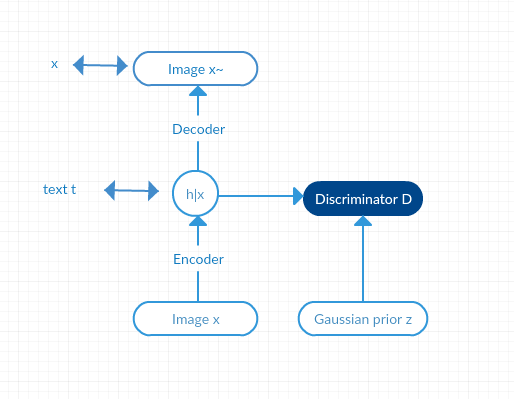
\includegraphics[height=2.30in]{fig1}
        \caption{}
            \label{fig:Architecturea}
    \end{subfigure}%
    ~ 
    \begin{subfigure}[t]{0.5\textwidth}
        \centering
        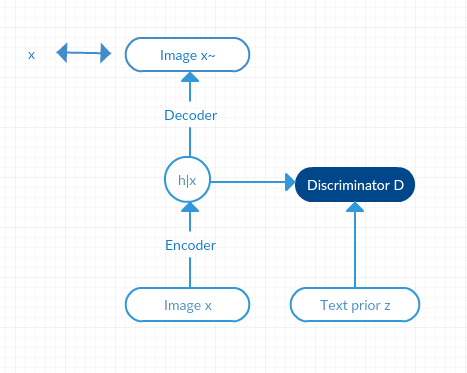
\includegraphics[height=2.30in]{fig2}
        \caption{}
                    \label{fig:Architectureb}
    \end{subfigure}
    \caption{Adversarial autoencoders with (a) Gaussian prior and explicit matching to the text representation, and (b) text representations as positive samples drawn from some underlying prior of text distribution.}
    \label{fig:Architecture}
\end{figure*}

% ----------------------------------------------------


% ----------------------------------------------------

\subsection{SAAE-imp}
\label{subsec:TextPrior}
	
	The implicit SAAE \ref{fig:Architectureb} takes the text representation $\bb{t}^c$ as the positive sample drawn from some underlying prior dictating the distribution of the text representation of a class. In this architecture, the code is driven to match the text representation through the adversarial net itself. The optimization problem for this learning scheme is of the same form as the standard adversarial autoencoder,
	\begin{align}
   L_{semantic} + \min_{G} \max_D E_{\bb{t} \sim r(\bb{t})}\left[\; \log D(\bb{t}) \;\right] + E_{\bb{x} \sim p_d(\bb{x})}\left[\; \log( 1 - D(G(\bb{x})) ) \;\right],
	\end{align}
	except that the prior serves as a guide to match the text distribution rather than as a regularizer that drives the encoding to match a Gaussian noise.


% ----------------------------------------------------

\subsection{SAE-GAN}

	We also check whether adding GAN to the original architecture of SAE will change the performance of SAE. We solve the following optimization problem,
	\begin{align}
		\min_{G} \max_D E_{\bb{z} \sim r(\bb{z})}\left[\; \log D(\bb{z}) \;\right] + E_{\bb{x} \sim p_d(\bb{x})}\left[\; \log( 1 - D(G_{\textrm{SAE}}(\bb{x})) ) + L_{\textrm{SAE}} \;\right],
	\end{align}
	where
	\begin{align}
		G_{\textrm{SAE}}(\bb{x}) = W \bb{x}.
	\end{align}




% ----------------------------------------------------

\subsection{Classification task}

	There are two scenarios for ZSL in image classification, namely standard ZSL and generalized ZSL. During training time, given training images $\bb{x}^c$ and their corresponding semantic representations $\bb{t}^c$ for $N_s$ seen classes $c$, the model learns to bridge the gap between $x^c$ and $t^c$. 
    
	During testing time, for standard ZSL, we are given images $\bb{x}^{uc}$ from $N_{us}$ unseen classes and semantic representations $\bb{t}^{uc}$ for those unseen classes without knowing the correspondence between $\bb{x}^{uc}$ and $\bb{t}^{uc}$. The task is to determine which unseen class each image belongs to. For generalized ZSL, the test images are not constrained to unseen classes: images from both seen and unseen classes can be used as test images and semantic representations for both classes should be provided.

During testing time, we follow the same classification method as in \cite{kodirov2017semantic}. The input test image $X$ is first projected using weight matrix $W$ to get the semantic representation $H$ and then the test class is decided by
\begin{equation}
	\min_i D(S_i, H),
\end{equation}
where $D$ is the distance function, which can be the negative cosine similarity or the Euclidean distance, We find that cosine similarity in general gives higher classification accuracy than the Euclidean distance does. We use the former in our experiments.


% ---------------------------------------------------------

\section{Datasets}

We conduct our experiments on two datasets. The first one is the Caltech-UCSD Birds 200-2011 dataset \cite{wah2011caltech}, with 200 categories of bird images. The total number of images is 11,788, and each class consists of about 40 to 80 images. The second dataset is AwA \cite{lampert2014attribute}, which consists of 30,475 images of 50 classes of animals.

Following the preprocessing steps taken in \cite{kodirov2017semantic}, for CUB dataset, we extract the 1024D activation from last pooling layer of Inception-v1 \cite{szegedy2015going} as our image features. For AwA dataset, we use the extracted 1024D features provided by \cite{kodirov2017semantic}. We use the attribute vector of each class as the semantic representation of the class. The dimensions of the attribute vectors are 312 and 85 for the CUB and AwA datasets, respectively.

For the standard ZSL tasks, following the description of \cite{kodirov2017semantic}, we withhold 10 and 50 classes as the unseen classes for AwA and CUB datasets, respectively. For the generalized ZSL tasks on the CUB dataset, we follow the description of \cite{Xian2017}%
\footnote{Since we do not have the information about the details of the splitting but only the number of instances in each split, we only follow roughly there number of instances used in each split, but not the exactly same split.}%
, using 7,125 training images from the 150 seen classes, and 4,663 test images from both 150 seen and 50 unseen classes. On the AwA dataset, we use 19,094 training images from the 40 seen classes, and 11,381 test images from both 40 seen and 10 unseen classes.

When we run our experiments, the image features and the attribute vectors are both normalized to $[0, 1]$ over the entire dataset.



% ---------------------------------------------------------

\section{Experiments}

We compare the results of our models with the Semantic Autoencoder (SAE) \cite{kodirov2017semantic}, the Joint Latent Semantic Embedding (JLSE) \cite{zhang2016zero}, and the Synthesized classifiers (Sync) \cite{changpinyo2016synthesized}. Due to the lack of an identical dataset, we decide to re-implement SAE to produce a reasonable baseline. It is worth noting that our implementation of SAE differs from that of \cite{kodirov2017semantic} in that we solve the optimization problem by gradient descent%
\footnote{We use the AdaGrad optimizer of TensorFlow.}%
in its original form, while in \cite{kodirov2017semantic} the problem is solved by first transforming it into a simpler linear equation. We find that the classification accuracy of the standard ZSL tasks using our implementation of SAE on both CUB and AwA datasets is lower than that reported in \cite{kodirov2017semantic} (see Table \ref{tab:StandardZSL}). Although we cannot reproduce the results in \cite{kodirov2017semantic}, we implement our models in the same framework which we use for implementing SAE, in the following discussion, we will therefore focus on comparing our results with our own implementation of SAE for self consistency. Table \ref{tab:StandardZSL} and \ref{tab:GeneralizedZSL} show the experimental results as well as the accuracy reported in \cite{kodirov2017semantic}.



\begin{table}[!htb]
\centering
\begin{tabular}{lrr}
\toprule
 & CUB & AwA \\
\midrule
SAAE-exp & 10.3 & 64.6 \\
SAAE-imp & 2.0 & 14.4 \\
SAE-dir & \bf{60.2} & 77.0 \\
SAE-GAN & 5.7 & \bf{78.5} \\
\midrule
SAE \cite{kodirov2017semantic} & 61.4 & 84.7 \\
JLSE \cite{zhang2016zero} & 41.8 & 80.5 \\
Sync \cite{changpinyo2016synthesized} & 54.4 & 72.9 \\
\bottomrule \\
\end{tabular}
\caption{Top-1 per-class accuracy (\%) of ZSL. SAAE-exp and SAAE-imp are the semantic adversarial autoencoder using Gaussian and attribute as priors, respectively. SAE-dir is our implementation of SAE which directly solve the optimization problem in its original form.}
\label{tab:StandardZSL}
\end{table}

\begin{table}[!htb]
\centering
\begin{tabular}{lrr}
\toprule
 & CUB & AwA \\
\midrule
SAAE-exp & \bf{17.8} & \bf{60.0} \\
SAAE-imp & 0.5 & 2.4 \\
SAE-dir & 7.0 & 53.8 \\
SAE-GAN & 6.9 & 54.0 \\
\bottomrule \\
\end{tabular}
\caption{Top-1 per-class accuracy (\%) of generalized ZSL. SAAE-exp and SAAE-imp are the semantic adversarial autoencoder using Gaussian and attribute as priors, respectively. SAE-dir is our implementation of SAE which directly solve the optimization problem in its original form.}
\label{tab:GeneralizedZSL}
\end{table}

In the experiments of SAAE with explicit matching, the coefficients of the matching, reconstruction, and GAN terms are all set to 1. We run for 100 epochs, and report the result top-1 per-class accuracy using negative cosine similarity as the distance at test time. The mean and standard deviation of the Gaussian priors are set to be the mean and standard deviation of the attributes of the dataset.

In the experiments of SAAE with implicit matching, the coefficient of the reconstruction term is 10 and that of the GAN is 1. We run for 100 epochs, and report the result top-1 per-class accuracy using negative cosine similarity as the distance at test time.

In the experiments of our implementation of SAE, we find that better performance is given when the coefficient of the matching loss is 100 and that of the reconstruction loss is 1. This indicates that the performance of SAE is mostly driven by the direct matching between the encoded representation from the image and the attribute vector, and is only marginally driven by the autoencoder.

%(wrong) the coefficients of the matching loss and the reconstruction loss are both set to 1. We run for 100 epochs, and report the result top-1 per-class accuracy using negative cosine similarity as the distance at test time.

We find that on the CUB dataset, SAAE with explicit matching achieves the best accuracy in both standard and generalized ZSL tasks. On the AwA dataset, our SAE implementation gives the best accuracy on both standard and generalized ZSL tasks.



% ----------------------------------------------

\section{Discussion}

% \subsection{SAE}

% In the experiment of our implementation of SAE, we find that the best results are achieved when the coefficients of the matching loss and the reconstruction loss are both set to 1 (compared to having much larger coefficient of the matching loss)


% One thing to notice is that the result of SAE is heavily affected by the $\lambda$ in the equation. If we set the $\lambda$ to be 1, the accuracy will stay around 5\% for AWA dataset. The result will only become close to the best result we have when the $\lambda$ is set to around 100000. After incorporating the adversarial part, the choice of $\lambda$ no longer matters: the accuracy will become close the the best result even we set the $\lambda$ to be 1. 



\subsection{SAAE-exp}
Our extension with adding adversarial part for the autoencoder does not improve the accuracy for the strict ZSL scenario. We experiment with a lot of other settings, such as adding more layers for autoencoder, changing the hidden dimensions of generator and discriminator for adversarial part, and different sampling strategies, such as sampling from hidden state to produce negative samples, as described in \cite{makhzani2015adversarial} section 2. None of them give any performance boost. 

We suspect the reason could be two-folded. The first reason is that the semantic features plays the essential role to the model. We also try ablation study that does not include the semantic space as constraints. In this case the model is just slightly better than random guess. This is expected since ZSL task usually deals with fine-grained image classification, and without the additional semantic space input, the models trained only based on image features are likely to have a poor result. However, the only way we figure out to incorporate the semantic features into the adversarial autoencoder is to minimize the l2 loss between the hidden state of the encoder and the semantic representation, and this major constraint bound the accuracy of the model. 

The second possible reason is that the prior is hard to pick for the semantic distribution. The prior serves to regularize the encoded samples so that the hidden state of an encoder is similar to the prior distribution we choose. In normal cases, for example alignDraw\cite{mansimov2015generating}, gaussian prior works fine. However, in out scenario, the output from encoder has to be close to the semantic space, thus our chosen prior has to resemble the distribution of the semantic space. As discussed before, the semantic space is the probability that one attribute appears in this class. If we view the attributes in the space of all possible classes, this is similar to a multinomial distribution. However, changing gaussian prior to multinomial distribution also does not work well. 

The SAAE-exp model performs the best in generalized classification task. We think this is as expected due to the nature of our task. Adversarial autoencoder is proposed to regularize the class distribution with a shape. This regularized shape is even more important in fine-grained classification task we are dealing with, where the difference of classes is very subtle. The regularized shape can give a better split between different classes, and this will help improve the classification accuracy in generalized ZSL scenario.

\subsection{SAAE-imp}

We observe that the classification accuracy using SAAE with the attribute as the prior is very low in all experiments. The reason is that using attribute vectors as the prior only encourages the encoding to have the same distribution as that of the attributes, but not educating the encoder to learn how to generate the encoding such that each component of the encoding can best match its corresponding component of the attribute vector. Since each component of the attribute vector has very specific meaning, and at test time we predict the class label by matching each component of the given attribute vector with the corresponding component of the encoding generated from the test image, lacking the ability to correctly predict each component of the attribute vector leads to the poor performance of this approach.


\subsection{SAE-GAN}

By adding GAN on top of the SAE, we find that on the AwA dataset it improves the accuracy, but on the CUB dataset it does not. For the standard ZSL on the AwA dataset, in which GAN makes the most significant improvement, we conduct more detailed experiments to check how accuracy changes by using different coefficients for the GAN. The results are shown in Table \ref{tab:SAEGAN}. We observe that with suitable coefficient, GAN slightly improves the accuracy, but if the coefficient of GAN is too large, it harms the performance.


\begin{table}[t]
\centering
\begin{tabular}{lccccc}
\toprule
GAN coefficient & $10^{-1}$ & $10^{-2}$ & $10^{-3}$ & $10^{-4}$ & 0 \\
Accuracy (\%) & 35.4 & 76.7 & 78.5 & 77.7 & 77.0 \\
\bottomrule \\
\end{tabular}
\caption{The top-1 per-class accuray of the standard ZSL on the AwA dataset, using different coefficients for the GAN in SAE-GAN.}
\label{tab:SAEGAN}
\end{table}


% ----------------------------------------------------
% ----------------------------------------------------

\section{Conclusion}

In this paper, we proposed to use the adversarial antoencoder framework incorporating semantic features as a solution to ZSL problem. Our method named semantic adversarial autoencoder(SAAE) projects the image representation into the semantic feature space with a discriminator matching the projection to a given prior. It achieves comparable accuracies on AWA and CUB datasets, especially in the generalized ZSL scenario. We also demonstrate that this new SAAE model is more robust than existing SAE model through extensive experiments. 


\newpage
% ----------------------------------------------------
% ----------------------------------------------------

\bibliographystyle{plain}
\bibliography{MachineLearning}

\end{document}
